\begin{question}
这是一首关于杰克和黛安的小曲,两个在美国中心地带长大的孩子。
游戏如下。
% \footnote{Cliff Bekar, Lewis and Clark College}
  \begin{table}[h!]
    \centering
    \setlength{\extrarowheight}{2pt}
    \begin{tabular}{*{5}{c|}}
      \multicolumn{2}{c}{} & \multicolumn{3}{c}{黛安} \\\cline{3-5}
      \multicolumn{1}{c}{} &     & $x$ & $y$ & $z$ \\\cline{2-5}
      \multirow{3}*{杰克}  & $a$ & 1,1 & 2,1 & 2,0 \\\cline{2-5}
                           & $b$ & 2,3 & 0,2 & 2,1 \\\cline{2-5}
                           & $c$ & 2,1 & 1,2 & 3,0 \\\cline{2-5}
    \end{tabular}
  \end{table}
\begin{tasks}
    \task (\points{6}) 如果杰克先行动,找出所有纯纳什策略组合及其结果。
    请详细说明并解释你的策略组合。
\end{tasks}
\begin{solution}
  \begin{tasks} 
    \task
    请参见下面的扩展形式博弈树。\\
    \begin{center}
      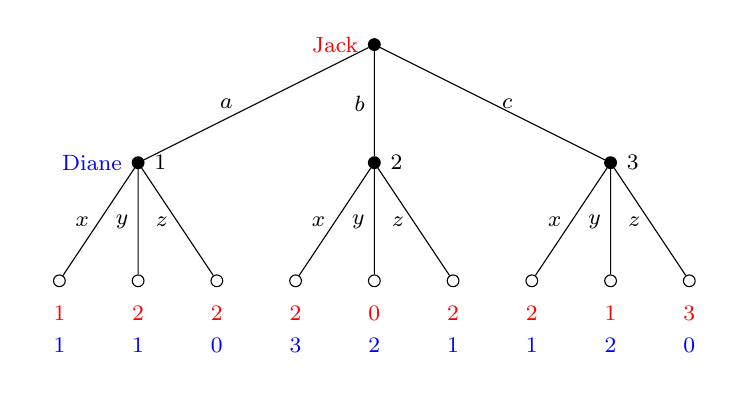
\begin{tikzpicture}[font=\footnotesize]
    \tikzstyle{solid node}=[circle,draw,inner sep=1.5,fill=black]
    \tikzstyle{hollow node}=[circle,draw,inner sep=1.5]
    \tikzstyle{level 1}=[level distance=15mm,sibling distance=3cm]
    \tikzstyle{level 2}=[level distance=15mm,sibling distance=1cm]
    \tikzstyle{level 3}=[level distance=15mm,sibling distance=.5cm]
    
    \node(0)[solid node,label=left:{\color{red} Jack}]{}
        child{node(1)[solid node,label=left:{\color{blue} Diane },label=right:{$1$}]{}
            child{node[hollow node,label=below:{
                \begin{tabular}{c}
                     {\color{red} 1}  \\
                     {\color{blue} \boxed{1}} 
                \end{tabular}
            }]{} edge from parent[] node[left]{$x$}}
            child{node[hollow node,label=below:{
                \begin{tabular}{c}
                  {\color{red} \boxed{2}}  \\
                     {\color{blue} \boxed{1}} 
                \end{tabular}
            }]{} edge from parent node[left]{$y$}}
            child{node[hollow node,label=below:{
                \begin{tabular}{c}
                     {\color{red} 2}  \\
                     {\color{blue} 0} 
                \end{tabular}
            }]{} edge from parent[ ] node[left]{$z$}}
            edge from parent node[left,xshift=-5]{$a$}
        }
        child{node(2)[solid node,label=right:{$2$}]{}
            child{node[hollow node,label=below:{
                \begin{tabular}{c}
                  {\color{red} \boxed{2}}  \\
                     {\color{blue} \boxed{3}} 
                \end{tabular}
            }]{} edge from parent[] node[left]{$x$}}
            child{node[hollow node,label=below:{
                \begin{tabular}{c}
                     {\color{red} 0}  \\
                     {\color{blue} 2} 
                \end{tabular}
            }]{} edge from parent[ ] node[left]{$y$}}
            child{node[hollow node,label=below:{
                \begin{tabular}{c}
                     {\color{red} 2}  \\
                     {\color{blue} 1} 
                \end{tabular}
            }]{} edge from parent[ ] node[left]{$z$}}
            edge from parent node[left]{$b$}
        }
        child{node(3)[solid node,label=right:{$3$}]{}
            child{node[hollow node,label=below:{
                \begin{tabular}{c}
                  {\color{red} \boxed{2}}  \\
                     {\color{blue} 1} 
                \end{tabular}
            }]{} edge from parent[ ] node[left]{$x$}}
            child{node[hollow node,label=below:{
                \begin{tabular}{c}
                     {\color{red} 1}  \\
                     {\color{blue} \boxed{2}} 
                \end{tabular}
            }]{} edge from parent[] node[left]{$y$}}
            child{node[hollow node,label=below:{
                \begin{tabular}{c}
                  {\color{red} \boxed{3}}  \\
                     {\color{blue} 0} 
                \end{tabular}
            }]{} edge from parent[ ] node[left]{$z$}}
            edge from parent node[right]{$c$}
        };
\end{tikzpicture}

    \end{center}
 
    \begin{itemize}

      \item 
      $\mathbf{N_1} = (\mathbf{a}, \ \mathbf{y_1} x_2 x_3 )$ 和
      $(\mathbf{a}, \mathbf{y_1}x_2y_3)$
      
      只要在节点3中黛安选择除$z$以外的任何策略,那么任何杰克选择$a$
      且黛安在节点$1$选择$y$的策略组合都是纳什均衡,因为给定对方的策略,双方都不会后悔。
      黛安在节点2总是选择$x$。

      该均衡的收益为$({\color{red} 2}, {\color{blue} 1})$

      \item 
        $\mathbf{N_2} = \left( \mathbf{b}, \ s_1 \mathbf{x_2} s_3 \right) $
      
      其中:
      \begin{itemize}
          \item $s_1$ 可以是 $\mathbf{x}$, $\mathbf{y}$; 
          \item $s_3$ 可以是 $\mathbf{x}$, $\mathbf{y}$ 或 $\mathbf{z}$。
      \end{itemize}

      任何策略组合中,只要杰克选择$b$,
      黛安在节点1(不在均衡路径上)对$x$和$y$无差异,
      且给定杰克选择$b$,黛安选择$x_2$。

      这些纳什策略组合的均衡结果
      为$({\color{red} 2}, {\color{blue} 3})$

    \end{itemize}

  \end{tasks}


\end{solution}
\end{question}
